Choosing an agent for real-world applications requires understanding the costs and resources needed for training and deployment, as well as the tradeoffs between different algorithms. To this end, our evaluation aims to answer three key questions. (\textbf{Q1}) How can data cost metrics be used in practice to compare methods that use offline data to those that do not? (\textbf{Q2}) How do system performance metrics inform training and deployment feasibility? (\textbf{Q3}) Can reliability metrics reveal tradeoffs between different agents that are not captured by raw task performance?

Our choice of baselines is guided by the action space of each domain. Circuit training and web navigation have discrete action spaces, so we evaluate them using DDQN and PPO, while quadruped locomotion has a continuous action space, so we use PPO and SAC. BC is included across all domains as an imitation learning baseline. For all domains and tasks, results are averaged over ten random seeds to ensure robustness and reproducibility. See Appendix \ref{appendix:additional_experiments} for more experimental results.



\subsection{\textbf{Q1}: Comparing Across Algorithm Types with Data Cost}\vspace{-0.2cm}
\textbf{\textit{How can data cost metrics be used in practice to compare methods that use offline data to those that do not?}}



\begin{figure}[!t]
    \centering
    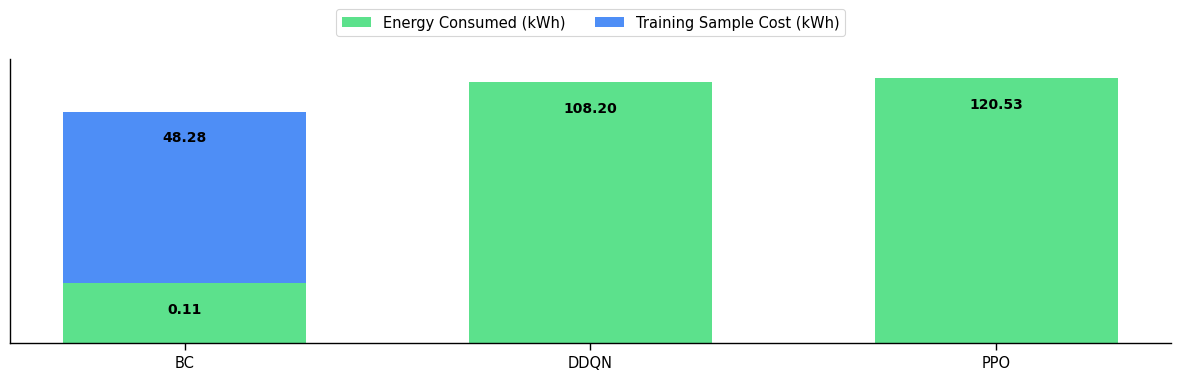
\includegraphics[width=1.0\linewidth]{img/ariane_data_cost_resize.png}
    \caption{Comparison of energy consumption and training sample cost for BC, DDQN, and PPO on the Ariane Netlist task, enabled by \method. \textbf{Note:} The plot is not to scale for visibility of smaller values. Online methods (DDQN and PPO) have no training sample cost as they are initialized without pre-collected data. BC's energy consumption (0.11 kWh) is significantly smaller than its training sample cost (48.28 kWh), which represents the energy used to generate the training data.}
    \label{fig:ariane_energy_comparison}
\end{figure}

\method provides datasets generated with agents of varying expertise (Section \ref{sec:training_sample_cost}), along with their associated training sample costs.
This enables the comparison of agents by considering both task performance and the cost of acquiring training data, which can vary significantly across different approaches like IL and RL.


Our experiments in the chip floorplanning domain reveal important insights about the true costs of different approaches. While BC's performance is competitive with DDQN and PPO (Table \ref{tab:metrics_circuit_training_ariane}), the training sample cost -- measured as the average energy consumed to train an agent that generates the data -- was $48.28$ kWh. In contrast, online methods like DDQN and PPO learn purely through environment interaction without requiring any pre-collected datasets, resulting in a training sample cost of zero.

The data cost metric allows researchers to combine the training sample cost with the energy consumed during training for a more comprehensive comparison. This approach provides a total energy cost that can be directly compared across offline, online, or hybrid methods. For example, offline training of a BC agent for the Ariane netlist consumed only 0.11 kWh. Therefore, the total energy cost for a BC agent would be $48.39$ kWh ($48.28$ kWh for generating the offline data + $0.11$ kWh for offline training).

When comparing total energy costs, we find that despite requiring pre-collected data, BC's total energy cost ($48.39$ kWh) is still lower than the energy consumed by online methods like DDQN and PPO, which amounted to $108.20$ kWh and $120.53$ kWh, respectively (Figure \ref{fig:ariane_energy_comparison}). For hybrid methods that use both offline data and online environment interactions, the total energy cost would similarly be calculated by adding the training sample cost for the offline data to the energy consumed during the online training phase.

These findings illustrate how data cost metrics can fundamentally change our understanding of algorithm efficiency. Without accounting for training sample costs, offline methods like BC would appear dramatically more efficient than online methods, potentially leading to misguided algorithm selection decisions. For domains with expensive data collection, like chip floorplanning where expert demonstrations may require considerable effort, the training sample cost metric becomes essential for fair comparisons. In contrast, for domains where high-quality data is readily available or inexpensive to collect, traditional online methods might remain preferable despite their higher training energy costs. 
% The data cost accounting framework in \method enables researchers and practitioners to make these nuanced decisions based on a complete understanding of the resource requirements across the entire agent development process.

\subsection{\textbf{Q2}: System Performance for Training and Deployment Feasibility}\vspace{-0.2cm}
\textbf{\textit{How do system performance metrics inform training and deployment feasibility?}}


\begin{figure}[!t]
    \centering
    \begin{subfigure}[b]{0.48\textwidth}
        \centering
        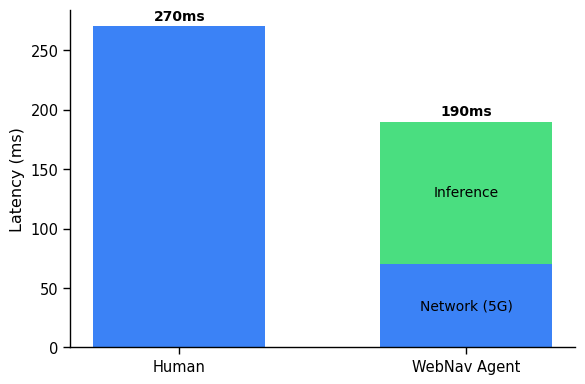
\includegraphics[width=\textwidth]{img/human_vs_webnav_agent.png}
        \caption{Comparison of web navigation agent latency with human reaction time. Agents are fast enough for real-time form-filling tasks, even when served from the cloud.}
        \label{fig:webnav-agent-latency}
    \end{subfigure}
    \hfill
    \begin{subfigure}[b]{0.38\textwidth}
        \centering
        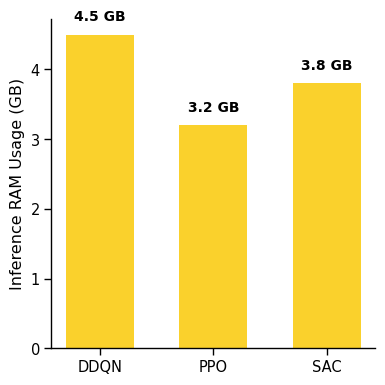
\includegraphics[width=\textwidth]{img/locomotion_ram_usage.png}
        \caption{Peak RAM usage for quadruped locomotion agents at inference time.}
        \label{fig:locomotion-ram-usage}
    \end{subfigure}
    \caption{System performance metrics for (a) Web Navigation agents and (b) Quadruped Locomotion agents. The latency comparison demonstrates the feasibility of real-time web interaction, while RAM usage highlights the resource requirements for deploying quadruped locomotion agents.}
    \label{fig:system-performance}
\end{figure}

Our experiments in the web navigation domain highlight the importance of considering hardware constraints and performance requirements of autonomous agents.
During training, PPO agents had a peak RAM usage of $2.3 \pm 0.14$ TB (Appendix Table \ref{tab:appendix_metrics_webnav_difficulty_1_websites_1}).
This high memory footprint can be attributed to the need for distributed experiments running hundreds of Google Chrome processes and storing batches of data, which involves tokenizing the entire DOM\footnote{\url{https://en.wikipedia.org/wiki/Document_Object_Model}} tree of HTML elements on each web page.
Such memory demands can limit the accessibility of training agents, as not all researchers may have access to the necessary hardware resources.
To put this into perspective, training a variant of the GPT-3 language model with approximately 72 billion parameters would require a similar amount of memory, assuming each parameter is stored as a 32-bit floating-point number \citep{brown2020language}.

However, the resource usage of these agents becomes more manageable for deployment.
The 120~ms inference time, when combined with the median round-trip latency of $\sim$68 ms for a 5G network \citep{schafhalter2023leveraging}, results in a total latency of $\sim$200 ms. This combined latency is still faster than the average human reaction time of $\sim$273 ms\footnote{\url{https://humanbenchmark.com/tests/reactiontime/statistics}}, enabling real-time responsiveness during web navigation tasks (Figure \ref{fig:webnav-agent-latency}).
Furthermore, the peak RAM usage of $2.19 \pm 0.09$ GB (Table \ref{tab:appendix_metrics_webnav_difficulty_1_websites_1}) indicates the feasibility of deploying trained agents directly on consumer-grade devices, such as smartphones, though the inference time may be slower on-device.

System performance metrics reveal critical practical constraints that might otherwise be overlooked during algorithm development.
The substantial gap between training and deployment resource requirements across our experiments demonstrates why evaluating both phases is essential. For web navigation agents, the extremely high training RAM requirements suggest that specialized infrastructure or algorithmic optimizations might be needed to make training more accessible to researchers with limited resources. Yet the reasonable inference requirements indicate these agents can be widely deployed once trained. This pattern (resource-intensive training but efficient inference) is common across many domains and highlights the importance of system performance metrics in guiding resource allocation decisions.
By explicitly measuring these metrics, \method helps researchers anticipate deployment constraints and identify potential bottlenecks early in the development process, facilitating more practical and deployable autonomous agents.

% \begin{figure}[!t]
%   \centering
%   \begin{minipage}[b]{0.53\linewidth}
%     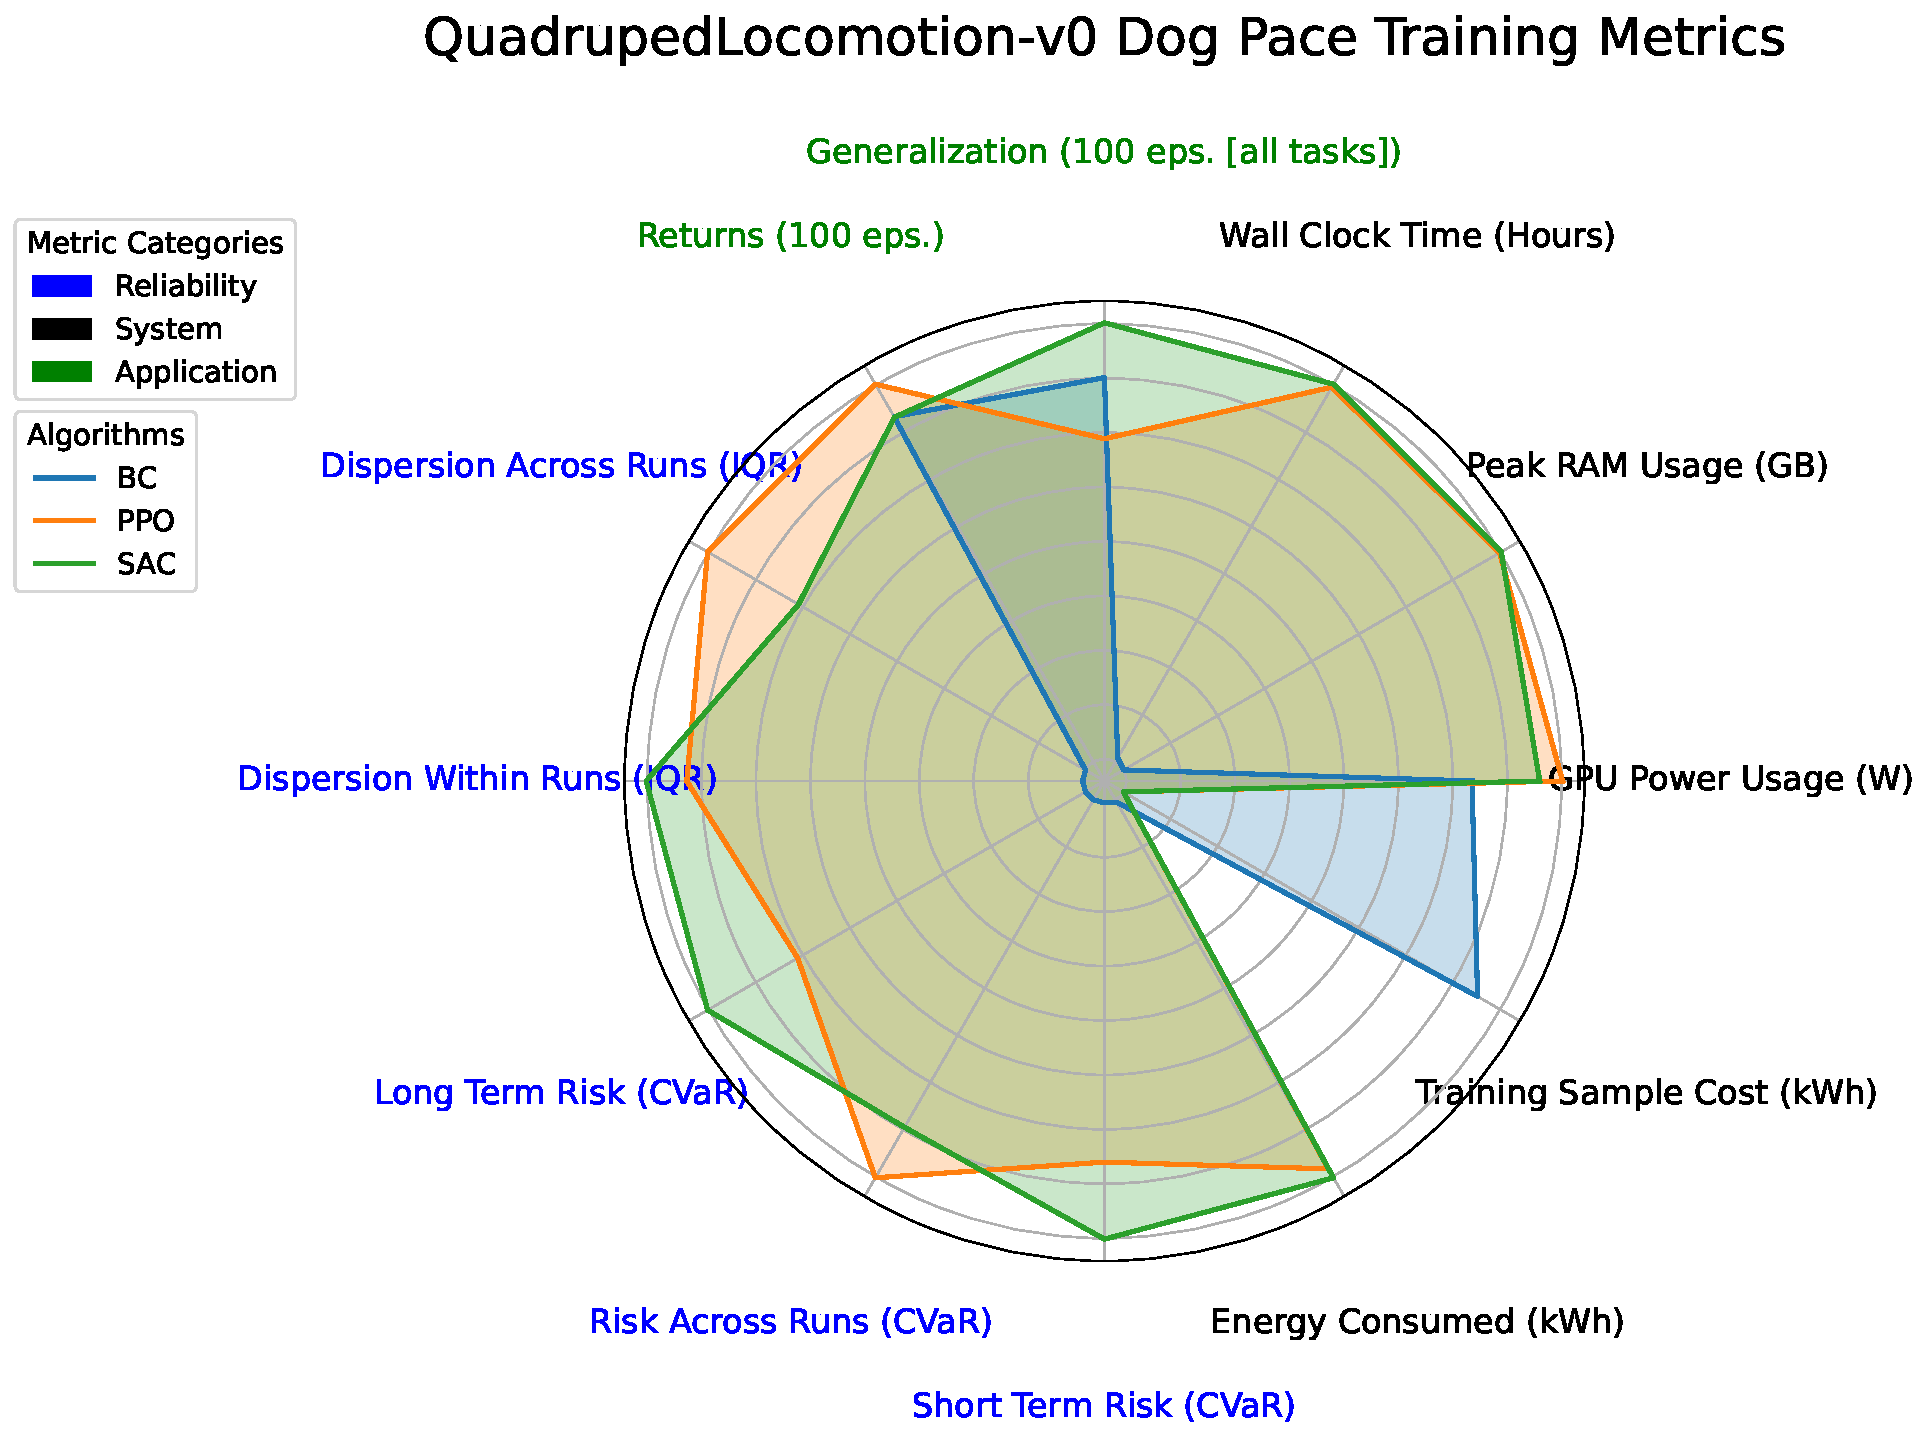
\includegraphics[width=\linewidth]{img/quadruped_locomotion/QuadrupedLocomotion-v0 Dog Pace Training Metrics.pdf}
%   \end{minipage}
%   \hfill % optional; adds horizontal spacing
%   \begin{minipage}[b]{0.4625\linewidth}
%     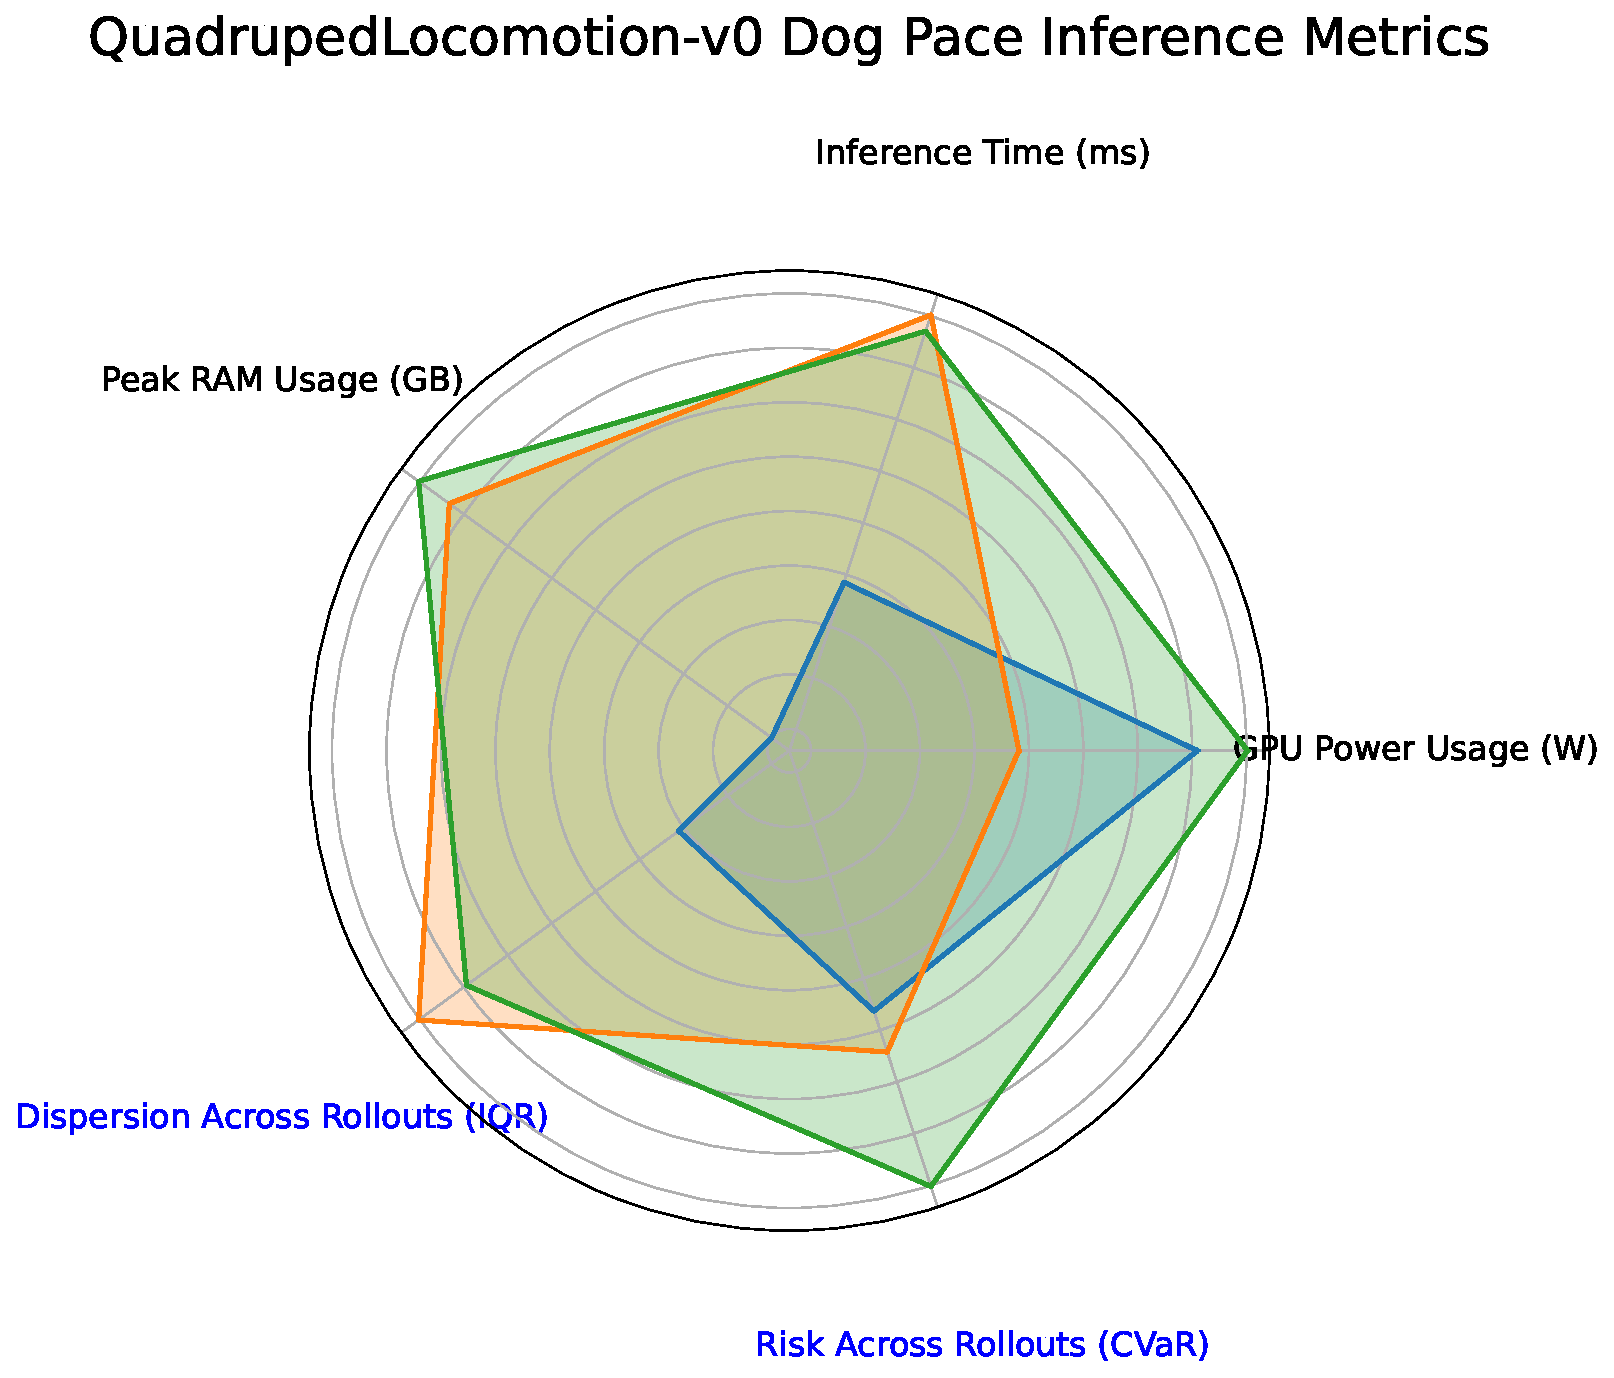
\includegraphics[width=\linewidth]{img/quadruped_locomotion/QuadrupedLocomotion-v0 Dog Pace Inference Metrics.pdf}
%   \end{minipage}
%   \caption{Graphical representation of metrics for the "dog pace" gait of QuadrupedLocomotion-v0}
%   \label{fig:radar_quadruped_locomotion_dog_pace}
% \end{figure}

% \subsection{Assessing Real-World Readiness through Reliability Metrics}
\subsection{\textbf{Q3}: Finding Tradeoffs with Reliability Metrics}\vspace{-0.2cm}
\textbf{\textit{Can reliability metrics reveal tradeoffs between different agents that are not captured by raw task performance?}}

\begin{figure}[!t]
    \centering
    \begin{subfigure}[b]{0.48\textwidth}
        \centering
        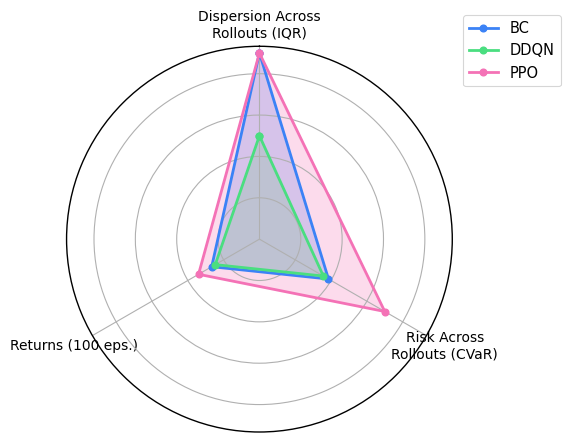
\includegraphics[width=\textwidth]{img/ariane_inference_reliability.png}
        \caption{Reliability metrics for chip floorplanning algorithms during inference on the Ariane netlist task. While task performance is similar between PPO and DDQN, PPO demonstrates better reliability metrics, providing a more consistent and predictable experience for human chip designers working with the generated layouts.}
        \label{fig:ariane-reliability}
    \end{subfigure}
    \hfill
    \begin{subfigure}[b]{0.48\textwidth}
        \centering
        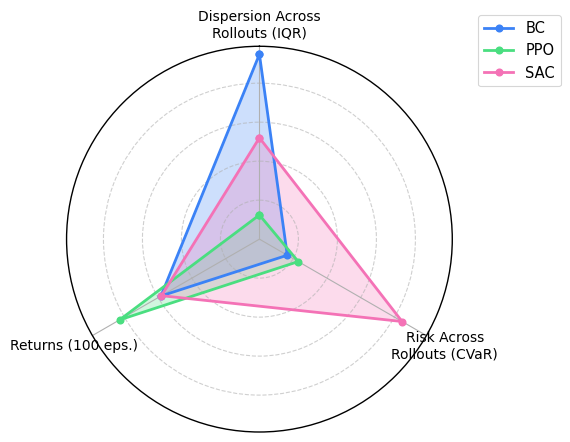
\includegraphics[width=\textwidth]{img/dog_pace_inference_reliability.png}
        \caption{Reliability metrics for quadruped locomotion algorithms during inference on the dog pace task. SAC shows notably better performance, achieving 3.7x better results than PPO in worst-case rollouts and demonstrating more consistent performance at inference time with 1.8x improvement in dispersion across rollouts.}
        \label{fig:dogpace-reliability}
    \end{subfigure}
    \caption{Comparison of reliability metrics across different domains and algorithms. The radar plots illustrate how different algorithms trade off between task performance and reliability.}
    \label{fig:reliability-comparison}
\end{figure}

Computer chip designers using autonomous agents rely on the agent to generate initial placements that they can build upon, so minimizing variability in the agent's performance is crucial.
As shown in Table \ref{tab:metrics_circuit_training_ariane}, the PPO algorithm exhibited lower dispersion across rollouts (IQR of \num{0.01}) compared to DDQN (IQR of \num{0.05}), indicating that PPO is approximately 5x more stable than DDQN when rolling out fixed, trained policies (Figure \ref{fig:ariane-reliability}).
This suggests that PPO would provide more consistent starting points for designers, enabling them to focus on refining and optimizing the floorplan instead of repeatedly rolling out the same policy to get similar initial placements.
Additionally, PPO demonstrated lower risk across rollouts (CVaR of $-1.01$) compared to DDQN (CVaR of $-1.25$), indicating that in the worst-performing rollouts, PPO performs about 1.2x better than DDQN on average, reducing the likelihood of designers starting with poor floorplans that require extensive manual adjustments.

In analyzing the ``Dog Pace" task of QuadrupedLocomotion-v0 (Table \ref{tab:appendix_locomotion_dog_pace}), we observe overlapping error bars on the returns for PPO and SAC.
To better understand their tradeoffs, we use the reliability metrics.
PPO provides a 2x reduction in both short-term and long-term risks compared to SAC, making PPO more stable.
This stability potentially makes PPO a safer option for training quadrupeds in the real world, where less sporadic behavior is needed.
Conversely, SAC performs 3.7x better than PPO in the worst-case rollouts on average and demonstrates a 1.8x improvement in dispersion across rollouts, indicating more consistent gaits during deployment -- essential from a safety perspective (Figure \ref{fig:dogpace-reliability}).

These reliability metrics provide insights that would be missed if we only considered task performance. For quadruped locomotion, the choice between PPO and SAC presents a clear tradeoff: PPO offers stability during training that could benefit researchers developing new control methods, while SAC provides more consistent performance during deployment that is crucial for real-world robot applications where unpredictable behaviors could damage hardware or create unsafe conditions. Similarly, in chip design, reliability metrics reveal PPO's advantage in producing consistent layouts—an attribute that significantly impacts user experience but isn't captured in typical performance metrics. Across domains, these findings demonstrate that reliability metrics are not merely statistical tools but practical indicators that directly relate to user experience, hardware safety, and development efficiency.
By evaluating algorithms through this lens, researchers can better align algorithm selection with the specific reliability requirements of their application domain.


\subsection{ Applying Metrics to Guide Real-World Algorithm Selection}\vspace{-0.2cm}


Our experimental evaluation across three domains demonstrates how different metrics in \method reveal complementary aspects of autonomous agent performance that are essential for real-world deployment decisions. While task performance provides a necessary baseline for comparison, the additional dimensions of data cost, system performance, and reliability metrics offer crucial insights for practitioners making algorithm selection decisions.

The relative importance of different metrics varies significantly by domain, reflecting different priorities in real-world applications.
For chip floorplanning, reliability metrics revealed PPO's advantage in providing consistent initial layouts—a property not evident from task performance alone but critical for human designers who need predictable starting points.
In web navigation, system performance metrics demonstrated that while training requires substantial compute resources, inference can be performed efficiently enough for real-time web interaction.
For quadruped locomotion, reliability metrics exposed a fundamental tradeoff between PPO's training stability and SAC's deployment stability that would be entirely missed by examining only average returns.

These findings illustrate \method's value as a comprehensive evaluation framework that enables informed algorithm selection based on application-specific priorities. Researchers developing new autonomous agent algorithms should consider which metrics matter most for their target domains: data-intensive applications may prioritize training sample cost, resource-constrained deployments might emphasize inference efficiency, safety-critical systems would focus on reliability metrics, and applications requiring adaptability would value generalization performance. By providing this multidimensional perspective, \method helps bridge the gap between algorithm development and successful real-world deployment of autonomous agents.